\documentclass[aspectratio=169,11pt]{beamer}

% TEMA Y COLORES
\usetheme{Madrid}
\usecolortheme{whale}

\definecolor{primaryblue}{RGB}{0,102,153}
\definecolor{accentgreen}{RGB}{0,128,0}
\definecolor{accentorange}{RGB}{204,102,0}
\definecolor{darkgray}{RGB}{64,64,64}

\setbeamercolor{palette primary}{bg=primaryblue,fg=white}
\setbeamercolor{palette secondary}{bg=primaryblue!80,fg=white}
\setbeamercolor{palette tertiary}{bg=primaryblue!60,fg=white}
\setbeamercolor{structure}{fg=primaryblue}
\setbeamercolor{block title}{bg=primaryblue,fg=white}
\setbeamercolor{block body}{bg=primaryblue!10}
\setbeamercolor{block title example}{bg=accentgreen,fg=white}
\setbeamercolor{block body example}{bg=accentgreen!10}
\setbeamercolor{block title alerted}{bg=accentorange,fg=white}
\setbeamercolor{block body alerted}{bg=accentorange!10}

% PAQUETES
\usepackage[utf8]{inputenc}
\usepackage[T1]{fontenc}
\usepackage{amsmath,amssymb}
\usepackage{booktabs}
\usepackage{tikz}
\usepackage{pgfplots}
\usepackage{listings}
\usepackage{multicol}

\pgfplotsset{compat=1.17}
\lstset{literate={ñ}{{\~n}}1 {á}{{\'a}}1 {é}{{\'e}}1 {í}{{\'i}}1 {ó}{{\'o}}1 {ú}{{\'u}}1}

% CÓDIGO PYTHON
\lstdefinestyle{pythonstyle}{
    language=Python,
    basicstyle=\ttfamily\footnotesize,
    keywordstyle=\color{blue}\bfseries,
    stringstyle=\color{red},
    commentstyle=\color{accentgreen}\itshape,
    frame=single,
    breaklines=true,
    showstringspaces=false,
    backgroundcolor=\color{gray!10}
}

% NAVEGACIÓN Y PIE DE PÁGINA
\setbeamertemplate{navigation symbols}{}
\setbeamertemplate{footline}{
    \leavevmode%
    \hbox{%
        \begin{beamercolorbox}[wd=.333333\paperwidth,ht=2.25ex,dp=1ex,center]{author in head/foot}%
            \usebeamerfont{author in head/foot}Matemáticas Financieras
        \end{beamercolorbox}%
        \begin{beamercolorbox}[wd=.333333\paperwidth,ht=2.25ex,dp=1ex,center]{title in head/foot}%
            \usebeamerfont{title in head/foot}Sesión 1
        \end{beamercolorbox}%
        \begin{beamercolorbox}[wd=.333333\paperwidth,ht=2.25ex,dp=1ex,right]{date in head/foot}%
            \usebeamerfont{date in head/foot}\insertframenumber{} / \inserttotalframenumber\hspace*{2ex}
        \end{beamercolorbox}}%
    \vskip0pt%
}

\title[Sesión 1]{Interés Simple e Interés Compuesto}
\subtitle{Fundamentos del valor del dinero en el tiempo}
\author{Matemáticas Financieras}
\institute{Valor del Dinero en el Tiempo}
\date{Semana 1 | Clase 1 | Duración: 1h 50min}

\begin{document}

% ===========================================
% SECCIÓN 1: PORTADA Y CONTENIDO
% ===========================================

\begin{frame}
    \titlepage
\end{frame}

\begin{frame}{Contenido de la Sesión}
    \tableofcontents
\end{frame}

% ===========================================
% SECCIÓN 2: INTRODUCCIÓN
% ===========================================
\section{Introducción}

\begin{frame}{Objetivos de Aprendizaje}
    Al finalizar esta sesión, serás capaz de:
    \begin{enumerate}
        \item Comprender por qué el dinero tiene valor en el tiempo
        \item Calcular interés simple y valor futuro con interés simple
        \item Derivar y aplicar la fórmula de interés compuesto
        \item Comparar el crecimiento lineal vs. exponencial del dinero
        \item Utilizar la HP 17bII+ y Python para cálculos financieros
    \end{enumerate}
\end{frame}

\begin{frame}{¿Por qué \$1 hoy vale más que \$1 mañana?}
    \begin{block}{Pregunta Inicial}
        Si te ofrecen \$10,000 hoy o \$10,000 dentro de un año, ¿cuál eliges?
    \end{block}

    \pause
    \vspace{0.5cm}

    \textbf{Tres razones fundamentales:}
    \begin{enumerate}
        \item<2-> \textbf{Costo de oportunidad}: Puedes invertir el dinero hoy
        \item<3-> \textbf{Inflación}: El poder adquisitivo disminuye con el tiempo
        \item<4-> \textbf{Riesgo}: El futuro es incierto
    \end{enumerate}

    \pause[5]
    \vspace{0.5cm}
    \begin{exampleblock}{Implicación}
        Para comparar flujos de dinero en diferentes momentos, necesitamos un \textbf{mecanismo de equivalencia}: las tasas de interés.
    \end{exampleblock}
\end{frame}

\begin{frame}{Definiciones Clave}
    \begin{block}{Principal ($P$)}
        Cantidad inicial de dinero invertida o prestada.
    \end{block}

    \begin{block}{Tasa de Interés ($r$ o $i$)}
        Precio del dinero expresado como porcentaje por período.
    \end{block}

    \begin{block}{Período ($n$)}
        Unidad de tiempo (años, meses, días) durante la cual se aplica el interés.
    \end{block}

    \begin{block}{Valor Futuro ($F$ o $FV$)}
        Valor del dinero en un momento posterior al presente.
    \end{block}
\end{frame}

% ===========================================
% SECCIÓN 3: DERIVACIONES MATEMÁTICAS
% ===========================================
\section{Interés Simple}

\begin{frame}{Interés Simple: Concepto}
    \begin{block}{Definición}
        En el \textbf{interés simple}, los intereses se calculan únicamente sobre el principal original, sin considerar intereses acumulados anteriormente.
    \end{block}

    \pause
    \vspace{0.5cm}

    \textbf{Característica clave:} El interés ganado en cada período es \textbf{constante}.

    \pause
    \vspace{0.5cm}

    \begin{exampleblock}{Ejemplo Conceptual}
        Si inviertes \$1,000 al 10\% anual simple:
        \begin{itemize}
            \item Año 1: Ganas \$100 de interés
            \item Año 2: Ganas \$100 de interés (sobre los \$1,000 originales)
            \item Año 3: Ganas \$100 de interés (sobre los \$1,000 originales)
        \end{itemize}
    \end{exampleblock}
\end{frame}

\begin{frame}{Derivación: Fórmula de Interés Simple}
    \textbf{Paso 1:} El interés ganado en cada período es:
    \begin{align*}
        I_{\text{por período}} = P \cdot r
    \end{align*}

    \pause
    \textbf{Paso 2:} Después de $n$ períodos, el interés total es:
    \begin{align*}
        I_{\text{total}} = P \cdot r \cdot n
    \end{align*}

    \pause
    \textbf{Paso 3:} El valor futuro es el principal más el interés:
    \begin{align*}
        F &= P + I_{\text{total}} \\
        F &= P + P \cdot r \cdot n \\
        F &= P(1 + r \cdot n)
    \end{align*}

    \pause
    \begin{block}{Fórmula de Interés Simple}
        \[
        \boxed{F = P(1 + rn)}
        \]
        donde $I = Prn$ es el interés total ganado.
    \end{block}
\end{frame}

\begin{frame}{Interés Simple: Crecimiento Lineal}
    \begin{columns}
        \begin{column}{0.5\textwidth}
            \textbf{Tabla de valores} (P = \$1,000, r = 10\%)

            \vspace{0.3cm}
            \begin{tabular}{@{}ccc@{}}
                \toprule
                $n$ & Interés & $F$ \\
                \midrule
                0 & \$0 & \$1,000 \\
                1 & \$100 & \$1,100 \\
                2 & \$200 & \$1,200 \\
                3 & \$300 & \$1,300 \\
                5 & \$500 & \$1,500 \\
                10 & \$1,000 & \$2,000 \\
                \bottomrule
            \end{tabular}
        \end{column}

        \begin{column}{0.5\textwidth}
            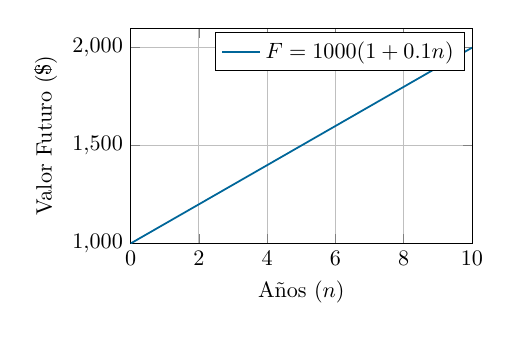
\begin{tikzpicture}[scale=0.8]
                \begin{axis}[
                    xlabel={Años ($n$)},
                    ylabel={Valor Futuro (\$)},
                    xmin=0, xmax=10,
                    ymin=1000, ymax=2100,
                    grid=major,
                    width=7cm,
                    height=5cm
                ]
                \addplot[color=primaryblue, thick, domain=0:10] {1000*(1+0.1*x)};
                \addlegendentry{$F = 1000(1+0.1n)$}
                \end{axis}
            \end{tikzpicture}

            \vspace{0.3cm}
            \textbf{Observación:} El crecimiento es \textcolor{primaryblue}{lineal}.
        \end{column}
    \end{columns}
\end{frame}

\section{Interés Compuesto}

\begin{frame}{Interés Compuesto: Concepto}
    \begin{block}{Definición}
        En el \textbf{interés compuesto}, los intereses se calculan sobre el principal \textbf{más} los intereses acumulados. Es decir, los intereses generan intereses.
    \end{block}

    \pause
    \vspace{0.5cm}

    \begin{alertblock}{La Magia del Interés Compuesto}
        ``El interés compuesto es la octava maravilla del mundo. El que lo entiende, lo gana; el que no, lo paga.'' --- Atribuido a Albert Einstein
    \end{alertblock}
\end{frame}

\begin{frame}{Derivación: Fórmula de Interés Compuesto (Paso a Paso)}
    Sea $P$ el principal y $r$ la tasa de interés por período.

    \pause
    \textbf{Al final del período 1:}
    \begin{align*}
        F_1 = P + P \cdot r = P(1 + r)
    \end{align*}

    \pause
    \textbf{Al final del período 2:}
    \begin{align*}
        F_2 = F_1 + F_1 \cdot r = F_1(1 + r) = P(1 + r)(1 + r) = P(1 + r)^2
    \end{align*}

    \pause
    \textbf{Al final del período 3:}
    \begin{align*}
        F_3 = F_2(1 + r) = P(1 + r)^2(1 + r) = P(1 + r)^3
    \end{align*}
\end{frame}

\begin{frame}{Derivación: Fórmula General}
    \textbf{Patrón general:} Al final del período $n$:
    \begin{align*}
        F_n = P(1 + r)^n
    \end{align*}

    \pause
    \vspace{0.5cm}

    \begin{block}{Fórmula de Interés Compuesto}
        \[
        \boxed{F = P(1 + r)^n}
        \]
    \end{block}

    \pause
    \vspace{0.3cm}

    \begin{exampleblock}{Componentes}
        \begin{itemize}
            \item $(1 + r)^n$ se llama \textbf{factor de capitalización}
            \item Representa cuántas veces se multiplica el principal
        \end{itemize}
    \end{exampleblock}
\end{frame}

\begin{frame}{Interés Compuesto: Crecimiento Exponencial}
    \begin{columns}
        \begin{column}{0.5\textwidth}
            \textbf{Tabla de valores} (P = \$1,000, r = 10\%)

            \vspace{0.3cm}
            \begin{tabular}{@{}ccc@{}}
                \toprule
                $n$ & Simple & Compuesto \\
                \midrule
                0 & \$1,000 & \$1,000 \\
                1 & \$1,100 & \$1,100 \\
                2 & \$1,200 & \$1,210 \\
                3 & \$1,300 & \$1,331 \\
                5 & \$1,500 & \$1,611 \\
                10 & \$2,000 & \$2,594 \\
                20 & \$3,000 & \$6,727 \\
                \bottomrule
            \end{tabular}
        \end{column}

        \begin{column}{0.5\textwidth}
            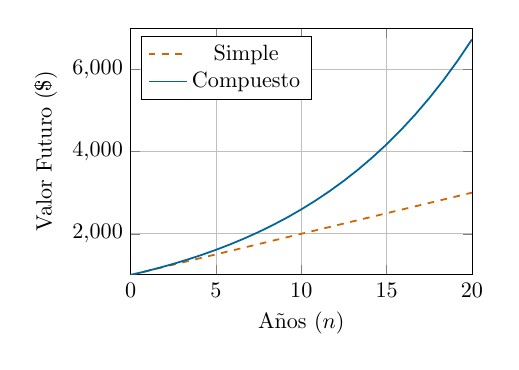
\begin{tikzpicture}[scale=0.8]
                \begin{axis}[
                    xlabel={Años ($n$)},
                    ylabel={Valor Futuro (\$)},
                    xmin=0, xmax=20,
                    ymin=1000, ymax=7000,
                    grid=major,
                    width=7cm,
                    height=5.5cm,
                    legend pos=north west
                ]
                \addplot[color=accentorange, thick, dashed, domain=0:20] {1000*(1+0.1*x)};
                \addlegendentry{Simple}
                \addplot[color=primaryblue, thick, domain=0:20] {1000*(1.1)^x};
                \addlegendentry{Compuesto}
                \end{axis}
            \end{tikzpicture}
        \end{column}
    \end{columns}

    \pause
    \vspace{0.3cm}
    \begin{alertblock}{Conclusión Clave}
        A largo plazo, el interés compuesto genera rendimientos \textbf{significativamente mayores}.
    \end{alertblock}
\end{frame}

\begin{frame}{Despejando las Variables}
    A partir de $F = P(1 + r)^n$, podemos despejar:

    \pause
    \vspace{0.3cm}

    \textbf{El Principal (Valor Presente):}
    \[
    \boxed{P = \frac{F}{(1 + r)^n}}
    \]

    \pause
    \vspace{0.3cm}

    \textbf{La Tasa de Interés:}
    \[
    \boxed{r = \left(\frac{F}{P}\right)^{1/n} - 1}
    \]

    \pause
    \vspace{0.3cm}

    \textbf{El Número de Períodos:}
    \[
    \boxed{n = \frac{\ln(F/P)}{\ln(1 + r)}}
    \]
\end{frame}

% ===========================================
% SECCIÓN 4: INTERPRETACIÓN VISUAL
% ===========================================
\section{Interpretación Visual}

\begin{frame}{Diagrama de Flujo de Caja}
    \begin{center}
        \begin{tikzpicture}[scale=1.2]
            % Línea de tiempo
            \draw[thick, ->] (0,0) -- (8,0) node[right] {Tiempo};

            % Marcas de tiempo
            \foreach \x/\label in {0/0, 2/1, 4/2, 6/n} {
                \draw (\x,0.1) -- (\x,-0.1) node[below] {\label};
            }

            % Puntos suspensivos
            \node at (5,0) {$\cdots$};

            % Flecha hacia abajo (inversión inicial)
            \draw[thick, ->, primaryblue] (0,0) -- (0,-1.5) node[below] {$-P$};

            % Flecha hacia arriba (valor futuro)
            \draw[thick, ->, accentgreen] (6,0) -- (6,1.5) node[above] {$+F$};

            % Anotaciones
            \node[align=center] at (0,-2.2) {\footnotesize Inversión\\inicial};
            \node[align=center] at (6,2.2) {\footnotesize Valor\\futuro};
        \end{tikzpicture}
    \end{center}

    \vspace{0.5cm}

    \begin{block}{Convención de Signos}
        \begin{itemize}
            \item \textcolor{primaryblue}{Flechas hacia abajo} (negativos): Salidas de dinero (inversiones, pagos)
            \item \textcolor{accentgreen}{Flechas hacia arriba} (positivos): Entradas de dinero (cobros, retornos)
        \end{itemize}
    \end{block}
\end{frame}

\begin{frame}{Comparación Visual: Simple vs. Compuesto}
    \begin{center}
        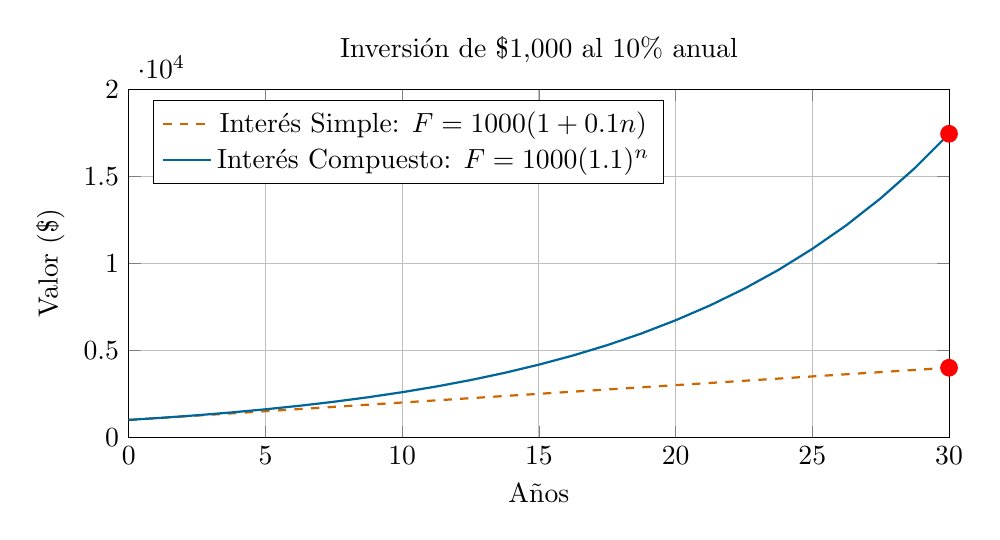
\begin{tikzpicture}
            \begin{axis}[
                xlabel={Años},
                ylabel={Valor (\$)},
                xmin=0, xmax=30,
                ymin=0, ymax=20000,
                grid=major,
                width=12cm,
                height=6cm,
                legend pos=north west,
                title={Inversión de \$1,000 al 10\% anual}
            ]
            \addplot[color=accentorange, thick, dashed, domain=0:30] {1000*(1+0.1*x)};
            \addlegendentry{Interés Simple: $F = 1000(1+0.1n)$}
            \addplot[color=primaryblue, thick, domain=0:30] {1000*(1.1)^x};
            \addlegendentry{Interés Compuesto: $F = 1000(1.1)^n$}

            % Punto de referencia
            \addplot[only marks, mark=*, mark size=3pt, color=red] coordinates {(30, 4000) (30, 17449)};
            \end{axis}
        \end{tikzpicture}
    \end{center}

    \pause
    En 30 años: Simple = \$4,000 vs. Compuesto = \$17,449. ¡Diferencia de \$13,449!
\end{frame}

\begin{frame}{El Poder del Tiempo}
    \begin{center}
        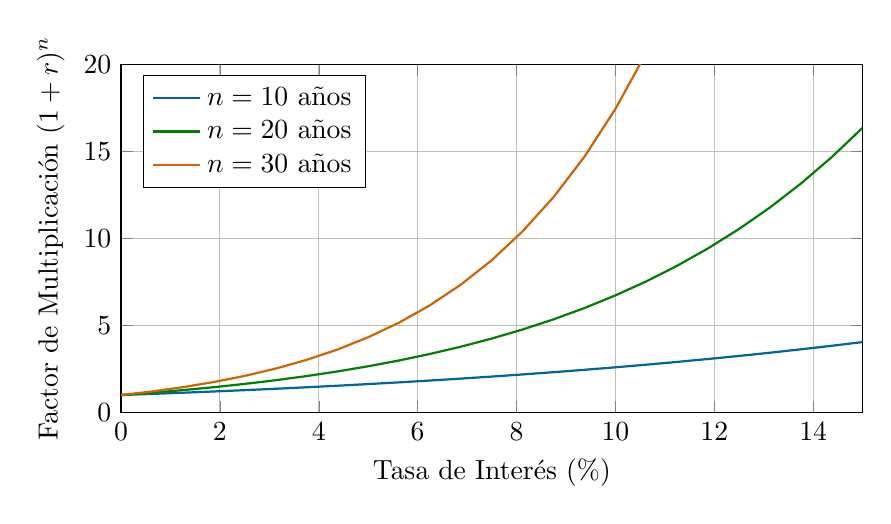
\begin{tikzpicture}
            \begin{axis}[
                xlabel={Tasa de Interés (\%)},
                ylabel={Factor de Multiplicación $(1+r)^n$},
                xmin=0, xmax=15,
                ymin=0, ymax=20,
                grid=major,
                width=11cm,
                height=6cm,
                legend pos=north west
            ]
            \addplot[color=primaryblue, thick, domain=0:15] {(1+x/100)^10};
            \addlegendentry{$n = 10$ años}
            \addplot[color=accentgreen, thick, domain=0:15] {(1+x/100)^20};
            \addlegendentry{$n = 20$ años}
            \addplot[color=accentorange, thick, domain=0:15] {(1+x/100)^30};
            \addlegendentry{$n = 30$ años}
            \end{axis}
        \end{tikzpicture}
    \end{center}

    \textbf{Observación:} El tiempo amplifica dramáticamente el efecto de la tasa de interés.
\end{frame}

% ===========================================
% SECCIÓN 5: TRUCOS DE ESTIMACIÓN
% ===========================================
\section{Trucos de Estimación Mental}

\begin{frame}{La Regla del 72}
    \begin{alertblock}{Regla del 72}
        Para estimar cuántos años tarda una inversión en \textbf{duplicarse}:
        \[
        \boxed{n \approx \frac{72}{r\%}}
        \]
        donde $r\%$ es la tasa de interés expresada en porcentaje.
    \end{alertblock}

    \pause
    \vspace{0.5cm}

    \textbf{Ejemplos rápidos:}
    \begin{itemize}
        \item Al 6\% anual: $n \approx 72/6 = 12$ años para duplicar
        \item Al 8\% anual: $n \approx 72/8 = 9$ años para duplicar
        \item Al 12\% anual: $n \approx 72/12 = 6$ años para duplicar
    \end{itemize}

    \pause
    \vspace{0.3cm}

    \begin{exampleblock}{Verificación}
        Al 8\%: $(1.08)^9 = 1.999 \approx 2$ \checkmark
    \end{exampleblock}
\end{frame}

\begin{frame}{¿Por qué 72?}
    La regla viene de resolver $2 = (1 + r)^n$ para $n$:
    \begin{align*}
        \ln(2) &= n \cdot \ln(1 + r) \\
        n &= \frac{\ln(2)}{\ln(1 + r)} \approx \frac{0.693}{r} \quad \text{(para $r$ pequeño)}
    \end{align*}

    \pause
    Multiplicando por 100: $n \approx \frac{69.3}{r\%}$

    \pause
    \vspace{0.3cm}

    \begin{alertblock}{¿Por qué usamos 72 y no 69?}
        \begin{itemize}
            \item 72 es divisible entre 2, 3, 4, 6, 8, 9, 12...
            \item Facilita el cálculo mental
            \item El error es mínimo para tasas entre 5\% y 15\%
        \end{itemize}
    \end{alertblock}
\end{frame}

\begin{frame}{Regla del 114 y del 144}
    \begin{alertblock}{Para triplicar: Regla del 114}
        \[
        \boxed{n_{\times 3} \approx \frac{114}{r\%}}
        \]
    \end{alertblock}

    \pause

    \begin{alertblock}{Para cuadruplicar: Regla del 144}
        \[
        \boxed{n_{\times 4} \approx \frac{144}{r\%}}
        \]
        Nota: $144 = 72 \times 2$ (duplicar dos veces = cuadruplicar)
    \end{alertblock}

    \pause
    \vspace{0.3cm}

    \textbf{Ejemplo:} Al 6\% anual:
    \begin{itemize}
        \item Duplicar: $72/6 = 12$ años
        \item Triplicar: $114/6 = 19$ años
        \item Cuadruplicar: $144/6 = 24$ años
    \end{itemize}
\end{frame}

\begin{frame}{Factores de Capitalización Útiles}
    \textbf{Memoriza estos valores para estimaciones rápidas:}

    \vspace{0.3cm}

    \begin{center}
    \begin{tabular}{@{}c|ccccc@{}}
        \toprule
        $r$ \textbackslash{} $n$ & 5 & 10 & 15 & 20 & 30 \\
        \midrule
        5\% & 1.28 & 1.63 & 2.08 & 2.65 & 4.32 \\
        8\% & 1.47 & 2.16 & 3.17 & 4.66 & 10.06 \\
        10\% & 1.61 & 2.59 & 4.18 & 6.73 & 17.45 \\
        12\% & 1.76 & 3.11 & 5.47 & 9.65 & 29.96 \\
        \bottomrule
    \end{tabular}
    \end{center}

    \pause
    \vspace{0.3cm}

    \begin{exampleblock}{Uso Rápido}
        ``¿Cuánto tendré si invierto \$5,000 al 10\% por 20 años?''

        $F \approx \$5,000 \times 6.73 = \$33,650$
    \end{exampleblock}
\end{frame}

% ===========================================
% SECCIÓN 6: CALCULADORA HP 17bII+
% ===========================================
\section{Calculadora HP 17bII+}

\begin{frame}{HP 17bII+: Navegación y Teclas Financieras}
    \textbf{Ruta:} \texttt{FIN} $\to$ \texttt{TVM} (menú principal financiero)

    \vspace{0.3cm}

    \begin{center}
        \begin{tabular}{@{}cl@{}}
            \toprule
            \textbf{Tecla (soft key)} & \textbf{Función} \\
            \midrule
            \texttt{N} & Número de períodos \\
            \texttt{I\%YR} & Tasa de interés \textbf{anual} nominal (\%) \\
            \texttt{PV} & Valor presente (Principal) \\
            \texttt{FV} & Valor futuro \\
            \texttt{PMT} & Pago periódico (no usado hoy) \\
            \texttt{P/YR} & Pagos por año (en \texttt{OTHER}) \\
            \texttt{+/-} & Cambiar signo \\
            \texttt{CLEAR DATA} & Borrar registros financieros \\
            \bottomrule
        \end{tabular}
    \end{center}

    \pause
    \vspace{0.3cm}

    \begin{alertblock}{Convención de Signos}
        \begin{itemize}
            \item Dinero que \textbf{sale} (inversión): \textbf{negativo} (usar \texttt{+/-})
            \item Dinero que \textbf{entra} (retorno): \textbf{positivo}
            \item \textbf{Importante:} Verificar que \texttt{P/YR = 1} para cálculos anuales
        \end{itemize}
    \end{alertblock}
\end{frame}

\begin{frame}{HP 17bII+: Ejemplo 1 - Calcular Valor Futuro}
    \begin{block}{Problema}
        Inviertes \$1,000 al 8\% anual compuesto por 5 años. ¿Cuál es el valor futuro?
    \end{block}

    \pause
    \vspace{0.3cm}

    \begin{center}
    \begin{tabular}{@{}lll@{}}
        \toprule
        \textbf{Teclas} & \textbf{Display} & \textbf{Descripción} \\
        \midrule
        \texttt{FIN} $\to$ \texttt{TVM} & & Entrar al menú TVM \\
        \texttt{CLEAR DATA} & 0.00 & Limpiar registros \\
        \texttt{1000 +/- PV} & -1,000.00 & Ingresa PV (negativo: sale) \\
        \texttt{8 I\%YR} & 8.00 & Tasa de interés 8\% anual \\
        \texttt{5 N} & 5.00 & 5 períodos \\
        \texttt{FV} & \textbf{1,469.33} & Calcula valor futuro \\
        \bottomrule
    \end{tabular}
    \end{center}

    \pause
    \vspace{0.3cm}

    \textbf{Verificación manual:} $F = 1000(1.08)^5 = 1000 \times 1.4693 = \$1,469.33$ \checkmark
\end{frame}

\begin{frame}{HP 17bII+: Ejemplo 2 - Calcular Tasa de Interés}
    \begin{block}{Problema}
        Una inversión de \$5,000 creció a \$8,000 en 6 años. ¿Cuál fue la tasa anual?
    \end{block}

    \pause
    \vspace{0.3cm}

    \begin{center}
    \begin{tabular}{@{}lll@{}}
        \toprule
        \textbf{Teclas} & \textbf{Display} & \textbf{Descripción} \\
        \midrule
        \texttt{CLEAR DATA} & 0.00 & Limpiar registros \\
        \texttt{5000 +/- PV} & -5,000.00 & Valor presente (sale) \\
        \texttt{8000 FV} & 8,000.00 & Valor futuro (entra) \\
        \texttt{6 N} & 6.00 & 6 períodos \\
        \texttt{I\%YR} & \textbf{8.15} & Calcula tasa de interés \\
        \bottomrule
    \end{tabular}
    \end{center}

    \pause
    \vspace{0.3cm}

    \textbf{Verificación:} $r = (8000/5000)^{1/6} - 1 = (1.6)^{0.1667} - 1 = 0.0815 = 8.15\%$ \checkmark
\end{frame}

\begin{frame}{HP 17bII+: Ejemplo 3 - Calcular Número de Períodos}
    \begin{block}{Problema}
        ¿Cuántos años tardará \$2,000 en convertirse en \$5,000 al 7\% anual?
    \end{block}

    \pause
    \vspace{0.3cm}

    \begin{center}
    \begin{tabular}{@{}lll@{}}
        \toprule
        \textbf{Teclas} & \textbf{Display} & \textbf{Descripción} \\
        \midrule
        \texttt{CLEAR DATA} & 0.00 & Limpiar registros \\
        \texttt{2000 +/- PV} & -2,000.00 & Valor presente \\
        \texttt{5000 FV} & 5,000.00 & Valor futuro \\
        \texttt{7 I\%YR} & 7.00 & Tasa 7\% anual \\
        \texttt{N} & \textbf{13.54} & Calcula períodos \\
        \bottomrule
    \end{tabular}
    \end{center}

    \pause
    \vspace{0.3cm}

    \textbf{Verificación:} $n = \frac{\ln(5000/2000)}{\ln(1.07)} = \frac{\ln(2.5)}{\ln(1.07)} = \frac{0.916}{0.0677} = 13.54$ años \checkmark
\end{frame}

% ===========================================
% SECCIÓN 7: EJERCICIOS PRÁCTICOS
% ===========================================
\section{Ejercicios Prácticos}

\begin{frame}{Ejercicio 1: Interés Simple}
    \begin{block}{Problema}
        Un préstamo de \$15,000 se otorga a una tasa de interés simple del 9\% anual. ¿Cuánto se debe pagar al final de 3 años?
    \end{block}

    \pause
    \vspace{0.3cm}

    \textbf{Solución:}
    \begin{align*}
        F &= P(1 + rn) \\
        F &= 15,000(1 + 0.09 \times 3) \\
        F &= 15,000(1 + 0.27) \\
        F &= 15,000 \times 1.27 \\
        F &= \$19,050
    \end{align*}

    \pause
    \textbf{Interés pagado:} $I = \$19,050 - \$15,000 = \$4,050$
\end{frame}

\begin{frame}{Ejercicio 2: Interés Compuesto}
    \begin{block}{Problema}
        Depositas \$25,000 en una cuenta que paga 6\% anual compuesto. ¿Cuánto tendrás después de 8 años?
    \end{block}

    \pause
    \vspace{0.3cm}

    \textbf{Solución:}
    \begin{align*}
        F &= P(1 + r)^n \\
        F &= 25,000(1.06)^8 \\
        F &= 25,000 \times 1.5938 \\
        F &= \$39,846.04
    \end{align*}

    \pause
    \vspace{0.3cm}

    \begin{exampleblock}{Verificación con Regla del 72}
        A 6\%, duplica en $72/6 = 12$ años. En 8 años debería ser más que \$25,000 pero menos que \$50,000. \checkmark
    \end{exampleblock}
\end{frame}

\begin{frame}{Ejercicio 3: Encontrar la Tasa}
    \begin{block}{Problema}
        Una inversión de \$10,000 se convirtió en \$16,000 en 5 años con capitalización anual. ¿Cuál fue la tasa de interés anual?
    \end{block}

    \pause
    \vspace{0.3cm}

    \textbf{Solución:}
    \begin{align*}
        F &= P(1 + r)^n \\
        16,000 &= 10,000(1 + r)^5 \\
        1.6 &= (1 + r)^5 \\
        (1.6)^{1/5} &= 1 + r \\
        1.0986 &= 1 + r \\
        r &= 0.0986 = 9.86\%
    \end{align*}

    \pause
    \textbf{Respuesta:} La tasa fue aproximadamente \textbf{9.86\% anual}.
\end{frame}

\begin{frame}{Ejercicio 4: Comparación Simple vs. Compuesto}
    \begin{block}{Problema}
        Tienes \$50,000 para invertir por 10 años. El Banco A ofrece 8\% simple anual. El Banco B ofrece 7\% compuesto anual. ¿Cuál es mejor?
    \end{block}

    \pause
    \vspace{0.3cm}

    \textbf{Banco A (Simple):}
    \begin{align*}
        F_A = 50,000(1 + 0.08 \times 10) = 50,000 \times 1.80 = \$90,000
    \end{align*}

    \pause
    \textbf{Banco B (Compuesto):}
    \begin{align*}
        F_B = 50,000(1.07)^{10} = 50,000 \times 1.9672 = \$98,358
    \end{align*}

    \pause
    \vspace{0.3cm}

    \begin{exampleblock}{Conclusión}
        El Banco B es mejor por \$8,358, a pesar de tener menor tasa nominal.
    \end{exampleblock}
\end{frame}

\begin{frame}{Ejercicio 5: Encontrar el Tiempo}
    \begin{block}{Problema}
        ¿En cuántos años se triplicará una inversión al 12\% anual compuesto?
    \end{block}

    \pause
    \vspace{0.3cm}

    \textbf{Solución exacta:}
    \begin{align*}
        3P &= P(1.12)^n \\
        3 &= (1.12)^n \\
        \ln(3) &= n \cdot \ln(1.12) \\
        n &= \frac{\ln(3)}{\ln(1.12)} = \frac{1.0986}{0.1133} = 9.69 \text{ años}
    \end{align*}

    \pause
    \vspace{0.3cm}

    \begin{alertblock}{Verificación con Regla del 114}
        $n \approx 114/12 = 9.5$ años. ¡Muy cercano! \checkmark
    \end{alertblock}
\end{frame}

% ===========================================
% SECCIÓN 8: PYTHON
% ===========================================
\section{Python con numpy-financial}

\begin{frame}[fragile]{Python: Instalación y Conceptos}
    \textbf{Instalación:}
    \begin{lstlisting}[style=pythonstyle]
pip install numpy-financial
    \end{lstlisting}

    \pause
    \vspace{0.3cm}

    \textbf{Funciones principales para esta sesión:}
    \begin{itemize}
        \item \texttt{npf.fv(rate, nper, pmt, pv)} -- Calcula valor futuro
        \item \texttt{npf.pv(rate, nper, pmt, fv)} -- Calcula valor presente
        \item \texttt{npf.rate(nper, pmt, pv, fv)} -- Calcula tasa
        \item \texttt{npf.nper(rate, pmt, pv, fv)} -- Calcula períodos
    \end{itemize}

    \pause
    \vspace{0.3cm}

    \begin{alertblock}{Convención de Signos (igual que HP 17bII+)}
        \begin{itemize}
            \item Dinero que sale: \textbf{negativo}
            \item Dinero que entra: \textbf{positivo}
            \item \texttt{pmt = 0} cuando no hay pagos periódicos
        \end{itemize}
    \end{alertblock}
\end{frame}

\begin{frame}[fragile]{Python: Ejercicio Completo}
    \begin{lstlisting}[style=pythonstyle]
import numpy_financial as npf

# Datos del problema
P = -1000    # Inversion inicial (negativo: sale)
r = 0.08     # Tasa 8% anual
n = 5        # 5 años

# Calcular valor futuro
F = npf.fv(rate=r, nper=n, pmt=0, pv=P)
print(f"Valor Futuro: ${F:,.2f}")

# Calcular tasa dado P, F, n
tasa = npf.rate(nper=n, pmt=0, pv=-1000, fv=1469.33)
print(f"Tasa calculada: {tasa*100:.2f}%")

# Calcular periodos para duplicar al 8%
periodos = npf.nper(rate=0.08, pmt=0, pv=-1, fv=2)
print(f"Periodos para duplicar: {periodos:.2f} años")
    \end{lstlisting}

    \pause
    \vspace{0.2cm}

    \textbf{Salida:}
\begin{verbatim}
Valor Futuro: $1,469.33
Tasa calculada: 8.00%
Periodos para duplicar: 9.01 años
\end{verbatim}
\end{frame}

\begin{frame}[fragile]{Python: Comparación Simple vs. Compuesto}
    \begin{lstlisting}[style=pythonstyle]
import numpy_financial as npf
import numpy as np

P = 10000  # Principal
r = 0.10   # Tasa 10%
años = np.arange(0, 31)

# Interes simple (formula manual)
F_simple = P * (1 + r * años)

# Interes compuesto (usando npf.fv)
F_compuesto = [-npf.fv(r, n, 0, -P) for n in años]

# Mostrar algunos valores
print("Año | Simple    | Compuesto")
print("-" * 35)
for n in [0, 5, 10, 20, 30]:
    print(f" {n:2d} | ${F_simple[n]:9,.2f} | ${F_compuesto[n]:9,.2f}")
    \end{lstlisting}
\end{frame}

% ===========================================
% SECCIÓN 9: RESUMEN Y TAREA
% ===========================================
\section{Resumen y Tarea}

\begin{frame}{Resumen de Fórmulas}
    \begin{columns}
        \begin{column}{0.5\textwidth}
            \textbf{Interés Simple}
            \begin{align*}
                F &= P(1 + rn) \\
                I &= Prn
            \end{align*}

            \vspace{0.5cm}

            \textbf{Interés Compuesto}
            \begin{align*}
                F &= P(1 + r)^n \\
                P &= \frac{F}{(1 + r)^n}
            \end{align*}
        \end{column}

        \begin{column}{0.5\textwidth}
            \textbf{Despeje de variables}
            \begin{align*}
                r &= \left(\frac{F}{P}\right)^{1/n} - 1 \\
                n &= \frac{\ln(F/P)}{\ln(1 + r)}
            \end{align*}

            \vspace{0.5cm}

            \textbf{Reglas de estimación}
            \begin{align*}
                n_{\times 2} &\approx 72/r\% \\
                n_{\times 3} &\approx 114/r\%
            \end{align*}
        \end{column}
    \end{columns}
\end{frame}

\begin{frame}{Conceptos Clave}
    \begin{enumerate}
        \item El dinero tiene \textbf{valor en el tiempo} por costo de oportunidad, inflación y riesgo
        \item \textbf{Interés simple}: crecimiento lineal, interés solo sobre el principal
        \item \textbf{Interés compuesto}: crecimiento exponencial, interés sobre interés
        \item A largo plazo, el compuesto supera significativamente al simple
        \item La \textbf{Regla del 72} permite estimaciones mentales rápidas
        \item Convención de signos: salidas (-), entradas (+)
    \end{enumerate}
\end{frame}

\begin{frame}{Tarea para la Próxima Sesión}
    \begin{enumerate}
        \item \textbf{Ejercicios HP 17bII+:}
        \begin{itemize}
            \item Calcular $F$ si $P = \$20,000$, $r = 9\%$, $n = 7$ años
            \item Calcular $n$ si $P = \$5,000$, $F = \$12,000$, $r = 11\%$
        \end{itemize}

        \vspace{0.3cm}

        \item \textbf{Problema:} Tienes la opción de recibir \$100,000 hoy o \$150,000 en 5 años. Si puedes invertir al 10\% anual compuesto, ¿cuál opción es mejor? Justifica matemáticamente.

        \vspace{0.3cm}

        \item \textbf{Python:} Escribe un programa que grafique el crecimiento de una inversión de \$1,000 al 5\%, 8\% y 12\% por 40 años.

        \vspace{0.3cm}

        \item \textbf{Reflexión:} ¿Por qué las instituciones financieras generalmente usan interés compuesto para préstamos e interés simple para algunos instrumentos de corto plazo?
    \end{enumerate}
\end{frame}

% ===========================================
% SECCIÓN 10: CIERRE
% ===========================================

\begin{frame}
    \begin{center}
        \Huge \textcolor{primaryblue}{\textbf{¿Preguntas?}}

        \vspace{1cm}
        \Large Próxima Sesión:\\
        \textbf{Valor Presente y Descuento}

        \vspace{0.5cm}
        \normalsize Semana 1, Clase 2
    \end{center}
\end{frame}

\end{document}
